% -*- root: Document.tex -*-

\chapter{Motivating Scenario}
\label{chap:motivation}

To illustrate and assess the benefits of proper container (or VM)\footnote{In the remaining of this document, we primarily consider containers, which are essentially lightweight VMs, and we use the two terms interchangeably.} placement, we first illustrate the limitation of existing scheduling policies on a simple scenario.

We define two types of containers: \emph{cpu-heavy} containers require 2 CPU cores and 1\,GB of RAM, while \emph{mem-heavy} containers require only 1 CPU core but 2\,GB of RAM.
We set up a cluster of nodes with 8 available cores and 8\,GB of RAM, running \textsc{Ubuntu Server} (v15.10) and \textsc{Docker} (v1.10.1).
The containers are managed by \text{Docker Swarm} (v1.2.0) and they execute the \textsc{stress-ng} benchmark~\cite{stress-ng} with a fixed total number of operations before terminating.

We deploy the containers in a dedicated cluster using four placement strategies:
\begin{itemize}
  \item \texttt{spread} places new containers on the node with the least number of containers;
  \item \texttt{binpack} deploys containers on the same node until its resources are totally exhausted before moving to the next node;
  \item \texttt{random} dispatches containers at random;
  \item \texttt{custom} assigns containers to nodes so that they fit into the least number of nodes, by taking into account both the CPU and memory requirements.
\end{itemize}

\begin{figure}[t]
  \centering
  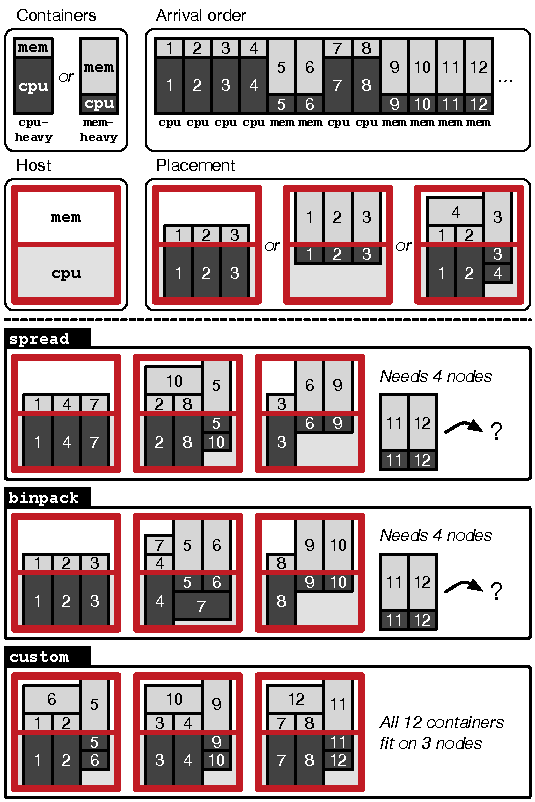
\includegraphics[width=.7\linewidth]{figures/scenario}
  \caption{Placement of the containers with 3 scheduling strategies for a given arrival order of containers, and assuming that a node can host 3 \emph{cpu-heavy} containers, or 3 \emph{mem-heavy} containers, or 2 of each type (top). While \texttt{spread} and \texttt{binpack} would require 4 nodes to schedule 12 containers, \texttt{custom} requires only 3 (bottom).}
  \label{fig:motivating-placement}
\end{figure}

For the sake of illustration, assume that a node can host \emph{(i)} 3 \emph{cpu-heavy}, or \emph{(ii)} 3 \emph{mem-heavy}, or \emph{(iii)} 2 \emph{cpu-heavy} and 2 \emph{mem-heavy} containers of each type.
In that case, a scheduler that takes into account the nature of the workload can obviously perform more efficient container placement.

Figure~\ref{fig:motivating-placement} shows a simple execution where the 12 containers (6 of each type) are registered in the following order: 4 \emph{cpu-heavy}, 2 \emph{mem-heavy}, 2 \emph{cpu-heavy}, 4 \emph{mem-heavy}.
Containers specify their resource needs and the system performs placement accordingly without overbooking.
A possible container scheduling for the \texttt{spread}, \texttt{binpack}, and \texttt{custom} strategies is shown in the bottom part of the figure.
As one can see, with 3 nodes available the first two strategies can only schedule 10 containers, whereas the \texttt{custom} strategy can place all of them on the 3 nodes.
Although very simplistic, this example illustrates the need for scheduling strategies that are aware of the requirements of the containers and the properties of the workloads.

\begin{figure}[t]
  \centering
  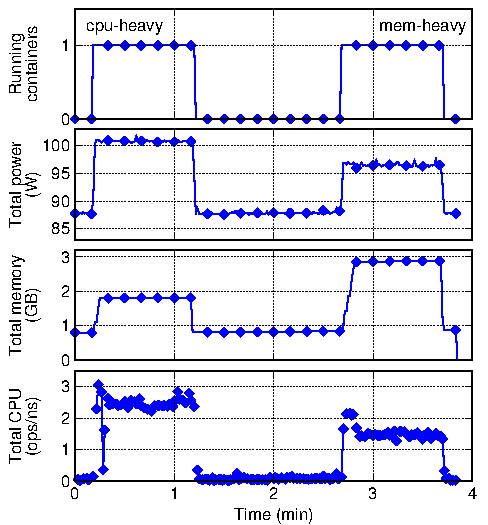
\includegraphics[width=.7\linewidth]{figures/plots/motivating_baseline/motivating_baseline}
  \caption{Workload for the two container types (\emph{cpu-heavy} and \emph{mem-heavy}) deployed on a single host.
  Each container runs for one minute, with an idle period in between.
  }
  \label{fig:motivating_baseline}
\end{figure}

In our actual experiment, we set the CPU load of containers to 20,000 ``bogo'' operations\footnote{Fake operations that represent the unit of load of the benchmark.} for each CPU core.
This corresponds to a total of $40,000$ and $20,000$ operations for \emph{cpu-heavy} and \emph{mem-heavy} containers, respectively.
Figure~\ref{fig:motivating_baseline} shows the baseline workloads induced by the two types of containers deployed on a single node, running one after the other within the span of $5$ minutes.
As expected, \emph{cpu-heavy} containers consume more energy---if we subtract the idle power, they require almost 50\% more than \emph{mem-heavy} containers---but they are less memory demanding.

Then, we design a more elaborated deployment scenario where we deploy start $20$ containers, alternating $5$ \emph{cpu-heavy} and $5$ \emph{mem-heavy}.
In all four deployment scenarios, we gather several measures (\emph{e.g.}, memory allocations, CPU usage, power consumptions).
Results are aggregated values over all nodes: number of CPU operations by time unit ($ns$), memory used in $GB$, and cumulative power (idle power and dynamic consumption) in $W$.
We observe that the \texttt{custom} strategy results in a more memory- and energy-efficient schedule because one of the nodes can be turned off---hence saving the idle power---without noticeably changing the number of operation executed---\emph{i.e.}, performance.

\begin{figure}[t]
  \centering
  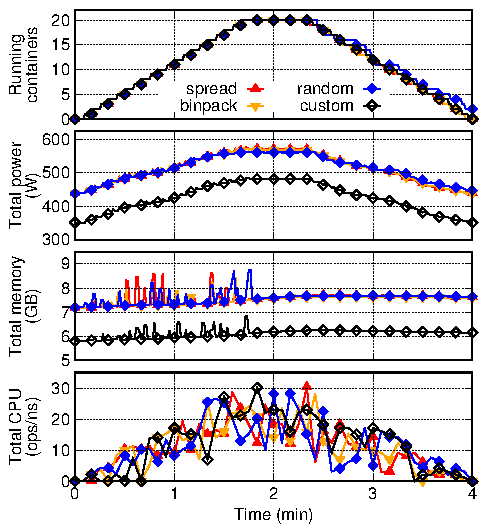
\includegraphics[width=.7\linewidth]{figures/plots/motivating/spread-binpack-random-custom}
  \caption{The \texttt{custom} strategy saves memory and energy without affecting performance thanks to more efficient container scheduling.}
  \label{fig:motivating}
\end{figure}

\newpage

As a summary, we aim at delivering a new container scheduler, \GP{}, that automatically learns from container's workloads to evenly distribute their deployment across a reduced number of nodes, thus drastically improving the power usage efficiency of a cluster.
As demonstrated, the state-of-the-art fails to achieve this objective as the \texttt{spread} strategy distributes the containers across all the nodes and \texttt{binpack} adopts a greedy heuristics to allocate containers node per node.
Given a set of available nodes $N$, we therefore aim at proposing a solution that minimizes the number of powered nodes required to host a set of containers $C$, thus ensuring that $|\text{genpack}(N,C)| \le |\text{binpack}(N,C)| \le |\text{spread}(N,C)| = |N|$, where $\text{f}(N,C)|$ indicates the number of nodes necessary for scheduling $C$ containers on $N$ nodes using algorithm $\text{f}$.
By doing so, \GP{} reduces the overall power consumption of a cluster without impacting the containers' performance, since hosts are not energy proportional (as shown in Figure~\ref{fig:motivating_baseline}).
